\apendice{Especificación de diseño}

\section{Introducción}

\section{Diseño de datos}

\subsection{Comparativa entre Bootstrap y Tailwind CSS}

En el diseño e implementación de la interfaz web del proyecto resulta necesario seleccionar un \textit{framework} de estilos que aporte productividad sin comprometer la mantenibilidad ni la calidad del código. Entre las alternativas más consolidadas se encuentran Bootstrap, orientado a componentes predefinidos, y Tailwind CSS, basado en un paradigma de utilidades. A continuación se presenta una comparativa crítica entre ambas opciones, justificando la elección final de Tailwind CSS para el desarrollo de esta página.

Bootstrap propone un conjunto amplio de componentes listos para usar, tales como barras de navegación, tarjetas o sistemas de rejilla, acompañados de un diseño visual relativamente homogéneo. Esta aproximación permite, en un primer momento, acelerar el desarrollo, ya que se pueden componer interfaces funcionales mediante la combinación de bloques estándar. Además, Bootstrap ofrece una documentación madura y una comunidad extensa, lo que facilita la resolución de dudas y la búsqueda de ejemplos; sin embargo, esta misma estandarización introduce ciertas limitaciones. Por un lado, la personalización profunda del diseño suele requerir sobrescribir reglas de estilo, lo que incrementa la complejidad de las hojas CSS y genera deuda técnica con facilidad. Por otro lado, las interfaces tienden a parecerse entre sí, de forma que la identidad visual del proyecto puede quedar diluida si no se realiza un esfuerzo considerable de adaptación.

En contraste, Tailwind CSS se basa en clases utilitarias de bajo nivel que describen propiedades concretas, tales como márgenes, tipografía o colores, aplicadas directamente sobre el marcado HTML. Esta filosofía permite construir componentes a medida a partir de combinaciones de utilidades, sin depender de un conjunto rígido de componentes predefinidos. Como consecuencia, el diseño resultante se ajusta mejor a los requisitos específicos del proyecto y favorece la creación de un sistema de diseño propio, más alineado con la identidad visual deseada. Además, Tailwind CSS integra mecanismos de purga de clases no utilizadas, lo que reduce de manera significativa el tamaño del fichero CSS final y mejora el rendimiento en producción.

No obstante, Tailwind CSS presenta también ciertos inconvenientes. Al inicio, la curva de aprendizaje puede parecer más pronunciada, ya que obliga a pensar en términos de propiedades de bajo nivel y no tanto en componentes cerrados. Asimismo, la presencia de múltiples clases en cada elemento puede dar lugar a un marcado aparentemente más denso, pero, cuando se interioriza el conjunto de utilidades y se adoptan buenas prácticas, como la extracción de componentes reutilizables y el uso de configuración centralizada, el resultado es un código más predecible y coherente, con menos necesidad de sobrescrituras complejas.

Desde una perspectiva de la ingeniería del software, la elección entre ambos enfoques afecta de forma directa a la mantenibilidad y escalabilidad del proyecto. Bootstrap ofrece rapidez inicial, pero puede derivar en hojas de estilo difíciles de gestionar cuando se requiere un alto grado de personalización. En cambio, Tailwind CSS promueve una relación más estrecha entre el diseño y el código, ya que el sistema de diseño se expresa mediante utilidades consistentes que se reutilizan en toda la aplicación. Esto reduce la duplicidad de estilos, minimiza el riesgo de efectos colaterales al modificar clases existentes y facilita la evolución del producto a largo plazo.

Finalmente, he optado por Tailwind CSS debido a su capacidad para generar interfaces más ligeras, a su enfoque modular y a su mejor integración con patrones modernos de desarrollo basado en componentes. Gracias a su sistema de utilidades, ha sido posible definir un diseño adaptado a las necesidades concretas del proyecto, mantener un control fino sobre el \textit{bundle} de estilos y reducir la deuda técnica asociada a la personalización del \textit{frontend}. En definitiva, Tailwind CSS proporciona un equilibrio más adecuado entre flexibilidad, rendimiento y mantenibilidad, lo que lo convierte en la opción más idónea para este desarrollo.

\begin{table}[h]
	\centering
	\renewcommand{\arraystretch}{1.3}
	\begin{tabular}{p{0.18\textwidth}p{0.36\textwidth}p{0.36\textwidth}}
		\hline
		\textbf{Aspecto} & \textbf{Bootstrap} & \textbf{Tailwind CSS} \\
		\hline
		Enfoque & Conjunto de componentes predefinidos y estilos de alto nivel &
		Clases utilitarias de bajo nivel que permiten construir componentes a medida \\
		\hline
		Curva de aprendizaje & Accesible al inicio gracias a los componentes estándar y a los ejemplos completos &
		Inicialmente más exigente, requiere pensar en términos de propiedades y sistemas de diseño \\
		\hline
		Productividad inicial & Elevada en prototipos y desarrollos con requisitos visuales genéricos &
		Crece con el tiempo, especialmente cuando se definen patrones reutilizables y componentes propios \\
		\hline
		Personalización del diseño & Personalización profunda costosa, necesidad frecuente de sobrescribir estilos y romper el diseño base &
		Alta capacidad de personalización mediante combinaciones de utilidades y configuración centralizada \\
		\hline
		Mantenibilidad & Riesgo de hojas CSS voluminosas y difíciles de refactorizar en proyectos muy adaptados &
		Estilos más controlados, menor necesidad de sobrescrituras y reducción de la deuda técnica \\
		\hline
		Rendimiento y tamaño del CSS & Tamaño mayor en el fichero final cuando se utilizan muchos componentes sin optimización específica &
		Tamaño significativamente reducido gracias a la purga de utilidades no utilizadas en el producto final \\
		\hline
		Identidad visual & Interfaces con aspecto reconocible y similar a otros proyectos basados en el mismo \textit{framework} &
		Mayor capacidad para definir una identidad visual propia y diferenciada \\
		\hline
		Comunidad y ecosistema & Comunidad muy amplia, gran cantidad de plantillas, ejemplos y recursos formativos &
		Comunidad en fuerte crecimiento, ecosistema consolidado en proyectos modernos basados en componentes \\
		\hline
	\end{tabular}
	\caption{Comparativa de ventajas e inconvenientes entre Bootstrap y Tailwind CSS}
	\label{tab:bootstrap_tailwind}
\end{table}

\section{Diseño arquitectónico}
\begin{figure}[h]
	\centering
	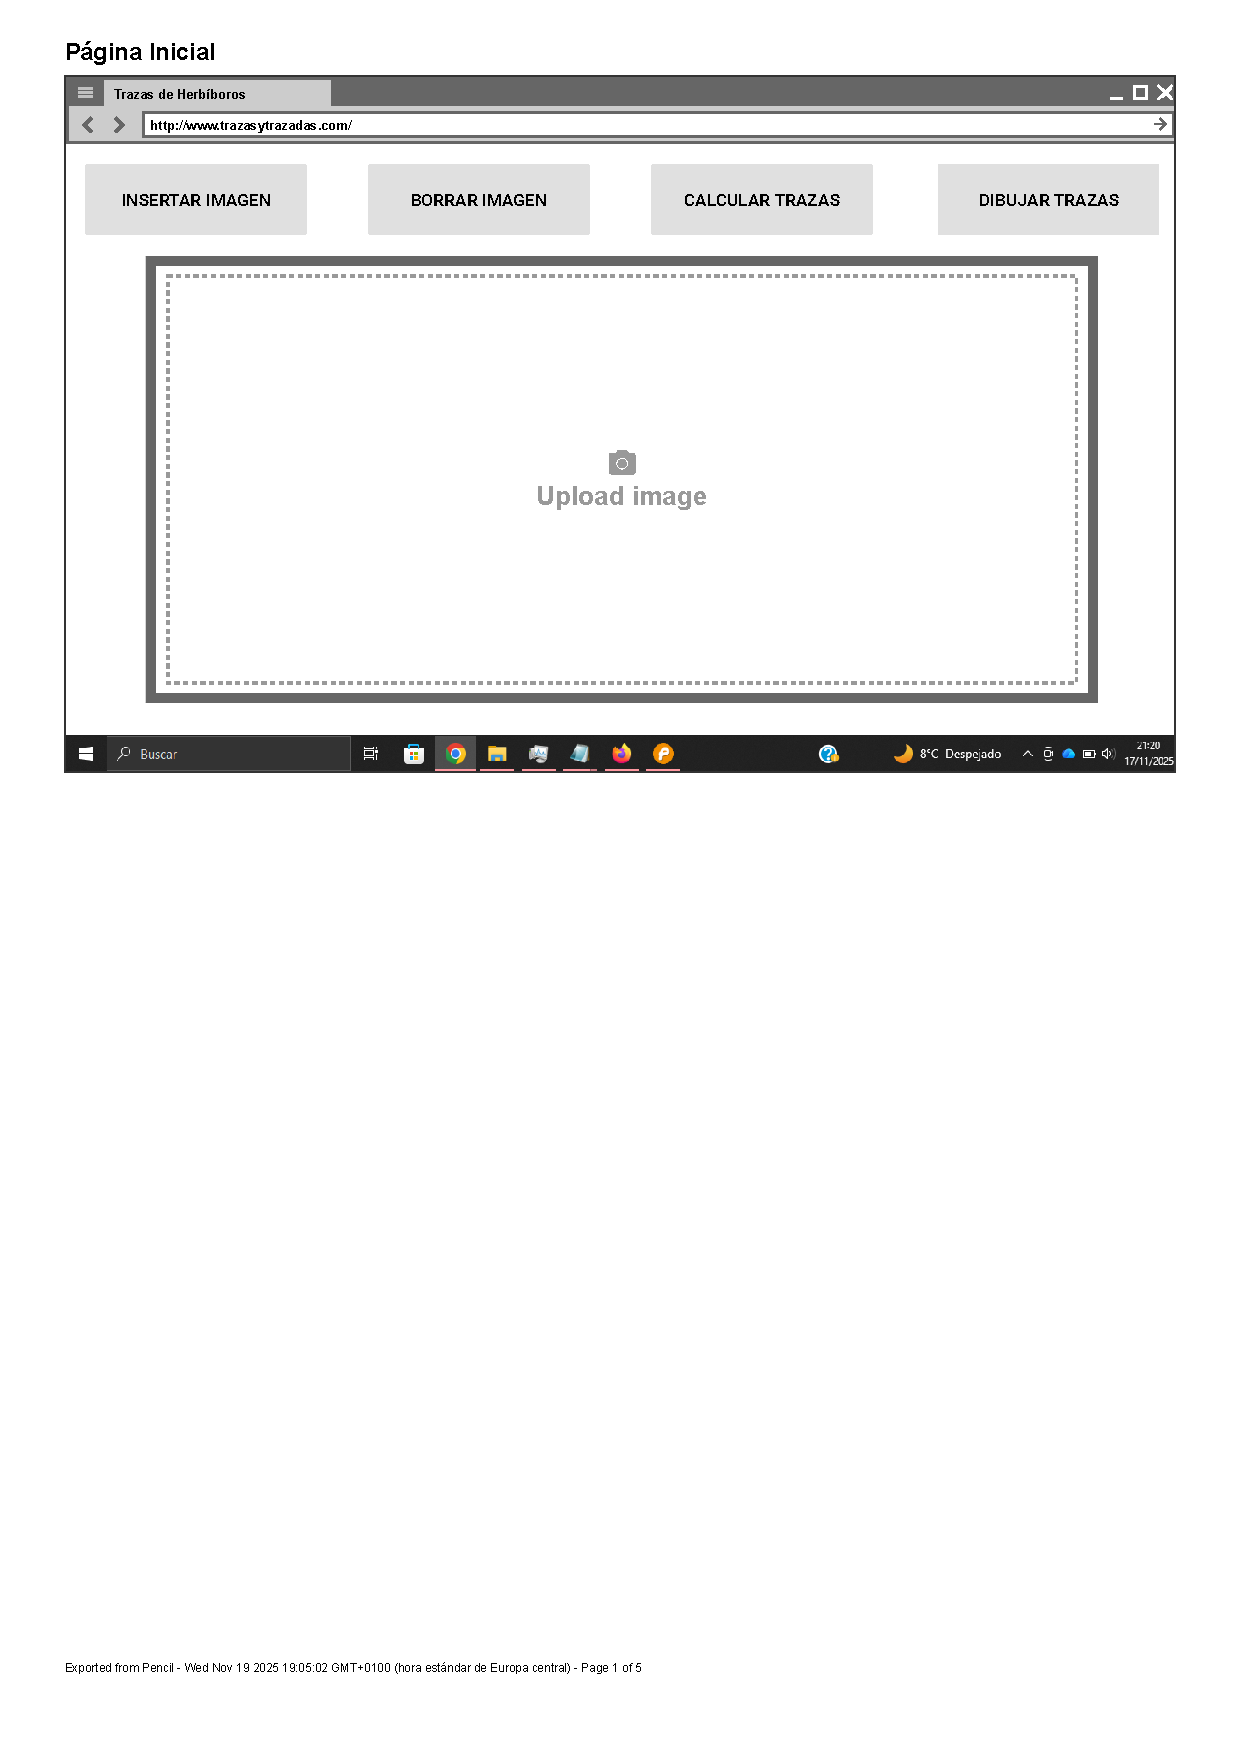
\includegraphics[width=\textwidth]{../assets/mockup/Mockup_web.pdf}
	\caption{Mockup de la web}
\end{figure}

\subsection{Arquitectura general de la aplicación}

\begin{figure}
	\centering
	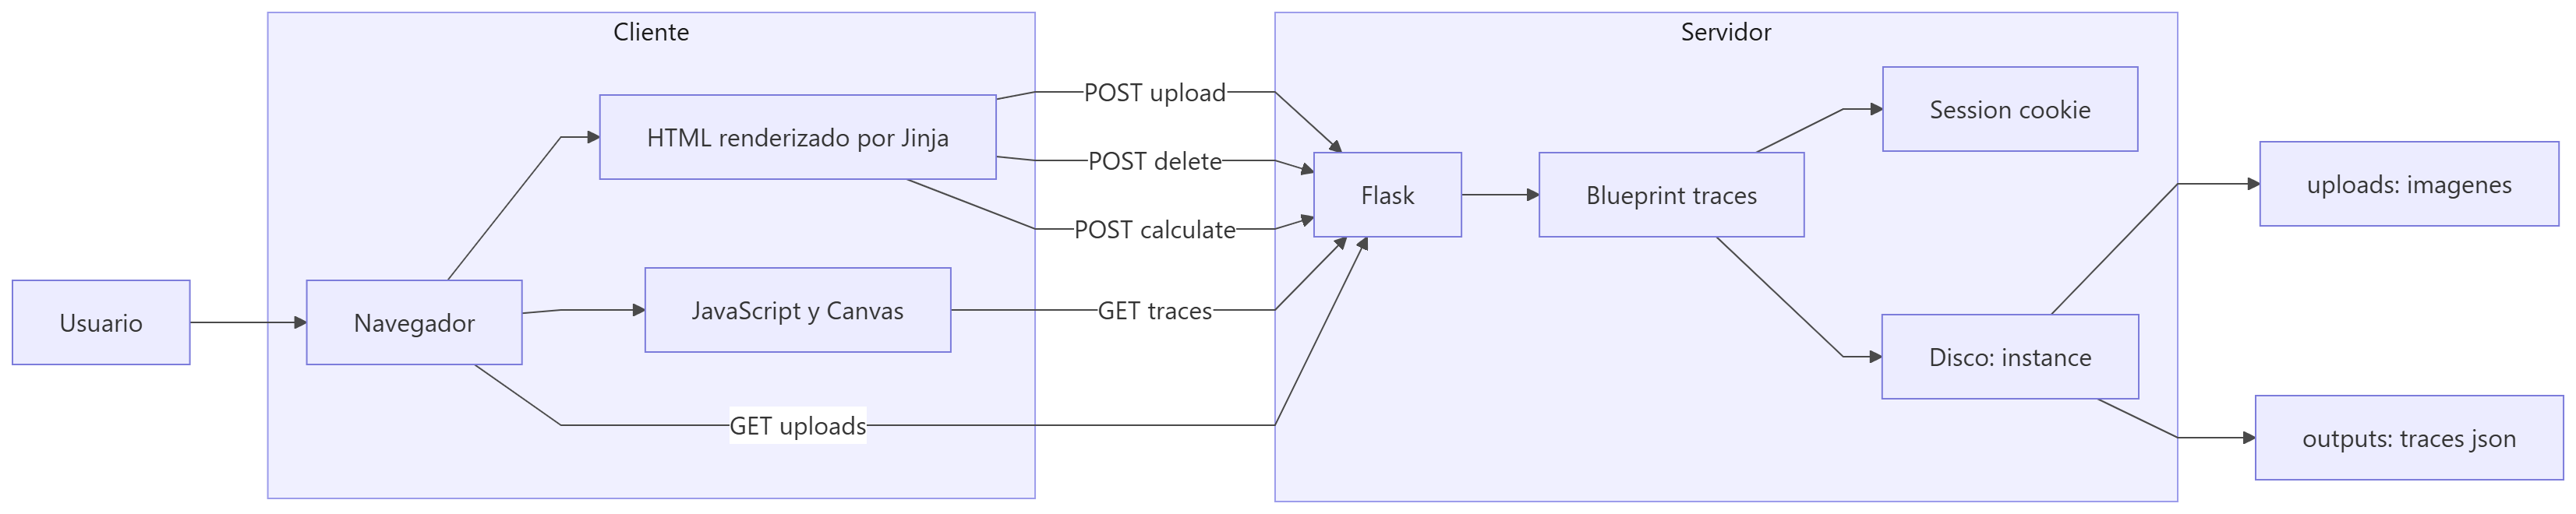
\includegraphics[width=0.7\linewidth]{img/diagrama_flujo}
	\caption[Diagrama de Flujo de la Aplicación]{}
	\label{fig:diagramaflujo}
\end{figure}


La Figura \ref{fig:diagramaflujo} representa la arquitectura general de la aplicación y las interacciones entre sus distintos componentes, diferenciando claramente el lado cliente y el lado servidor.

El usuario interactúa con la aplicación a través del navegador web, que actúa como intermediario entre la interfaz gráfica y el backend. En el cliente se distinguen dos responsabilidades bien separadas. Por un lado, el HTML renderizado mediante Jinja se encarga de mostrar la estructura de la interfaz, incluyendo botones, imágenes y modales informativos. Por otro lado, la lógica implementada en JavaScript, apoyada en un elemento \textit{canvas}, gestiona la descarga de los resultados en formato JSON y su representación gráfica, sin delegar operaciones de modificación visual al servidor.

El servidor, implementado con Flask, centraliza la lógica de negocio y expone los distintos endpoints a través de un \textit{Blueprint} dedicado a la gestión de trazas. Para mantener el estado de la aplicación entre peticiones HTTP, se utiliza una \textit{session cookie} que almacena información relativa a la imagen activa y a la disponibilidad de resultados calculados. Asimismo, el sistema emplea almacenamiento en disco, dentro del directorio \textit{instance}, tanto para persistir las imágenes subidas por el usuario como para guardar los resultados intermedios en formato JSON.

Este diseño garantiza una separación clara de responsabilidades, evitando que el cliente modifique directamente recursos en el servidor y relegando el procesamiento visual al navegador, lo que mejora la escalabilidad y simplifica la arquitectura.

\subsection{Flujo temporal de interacción entre componentes}

\begin{figure}
	\centering
	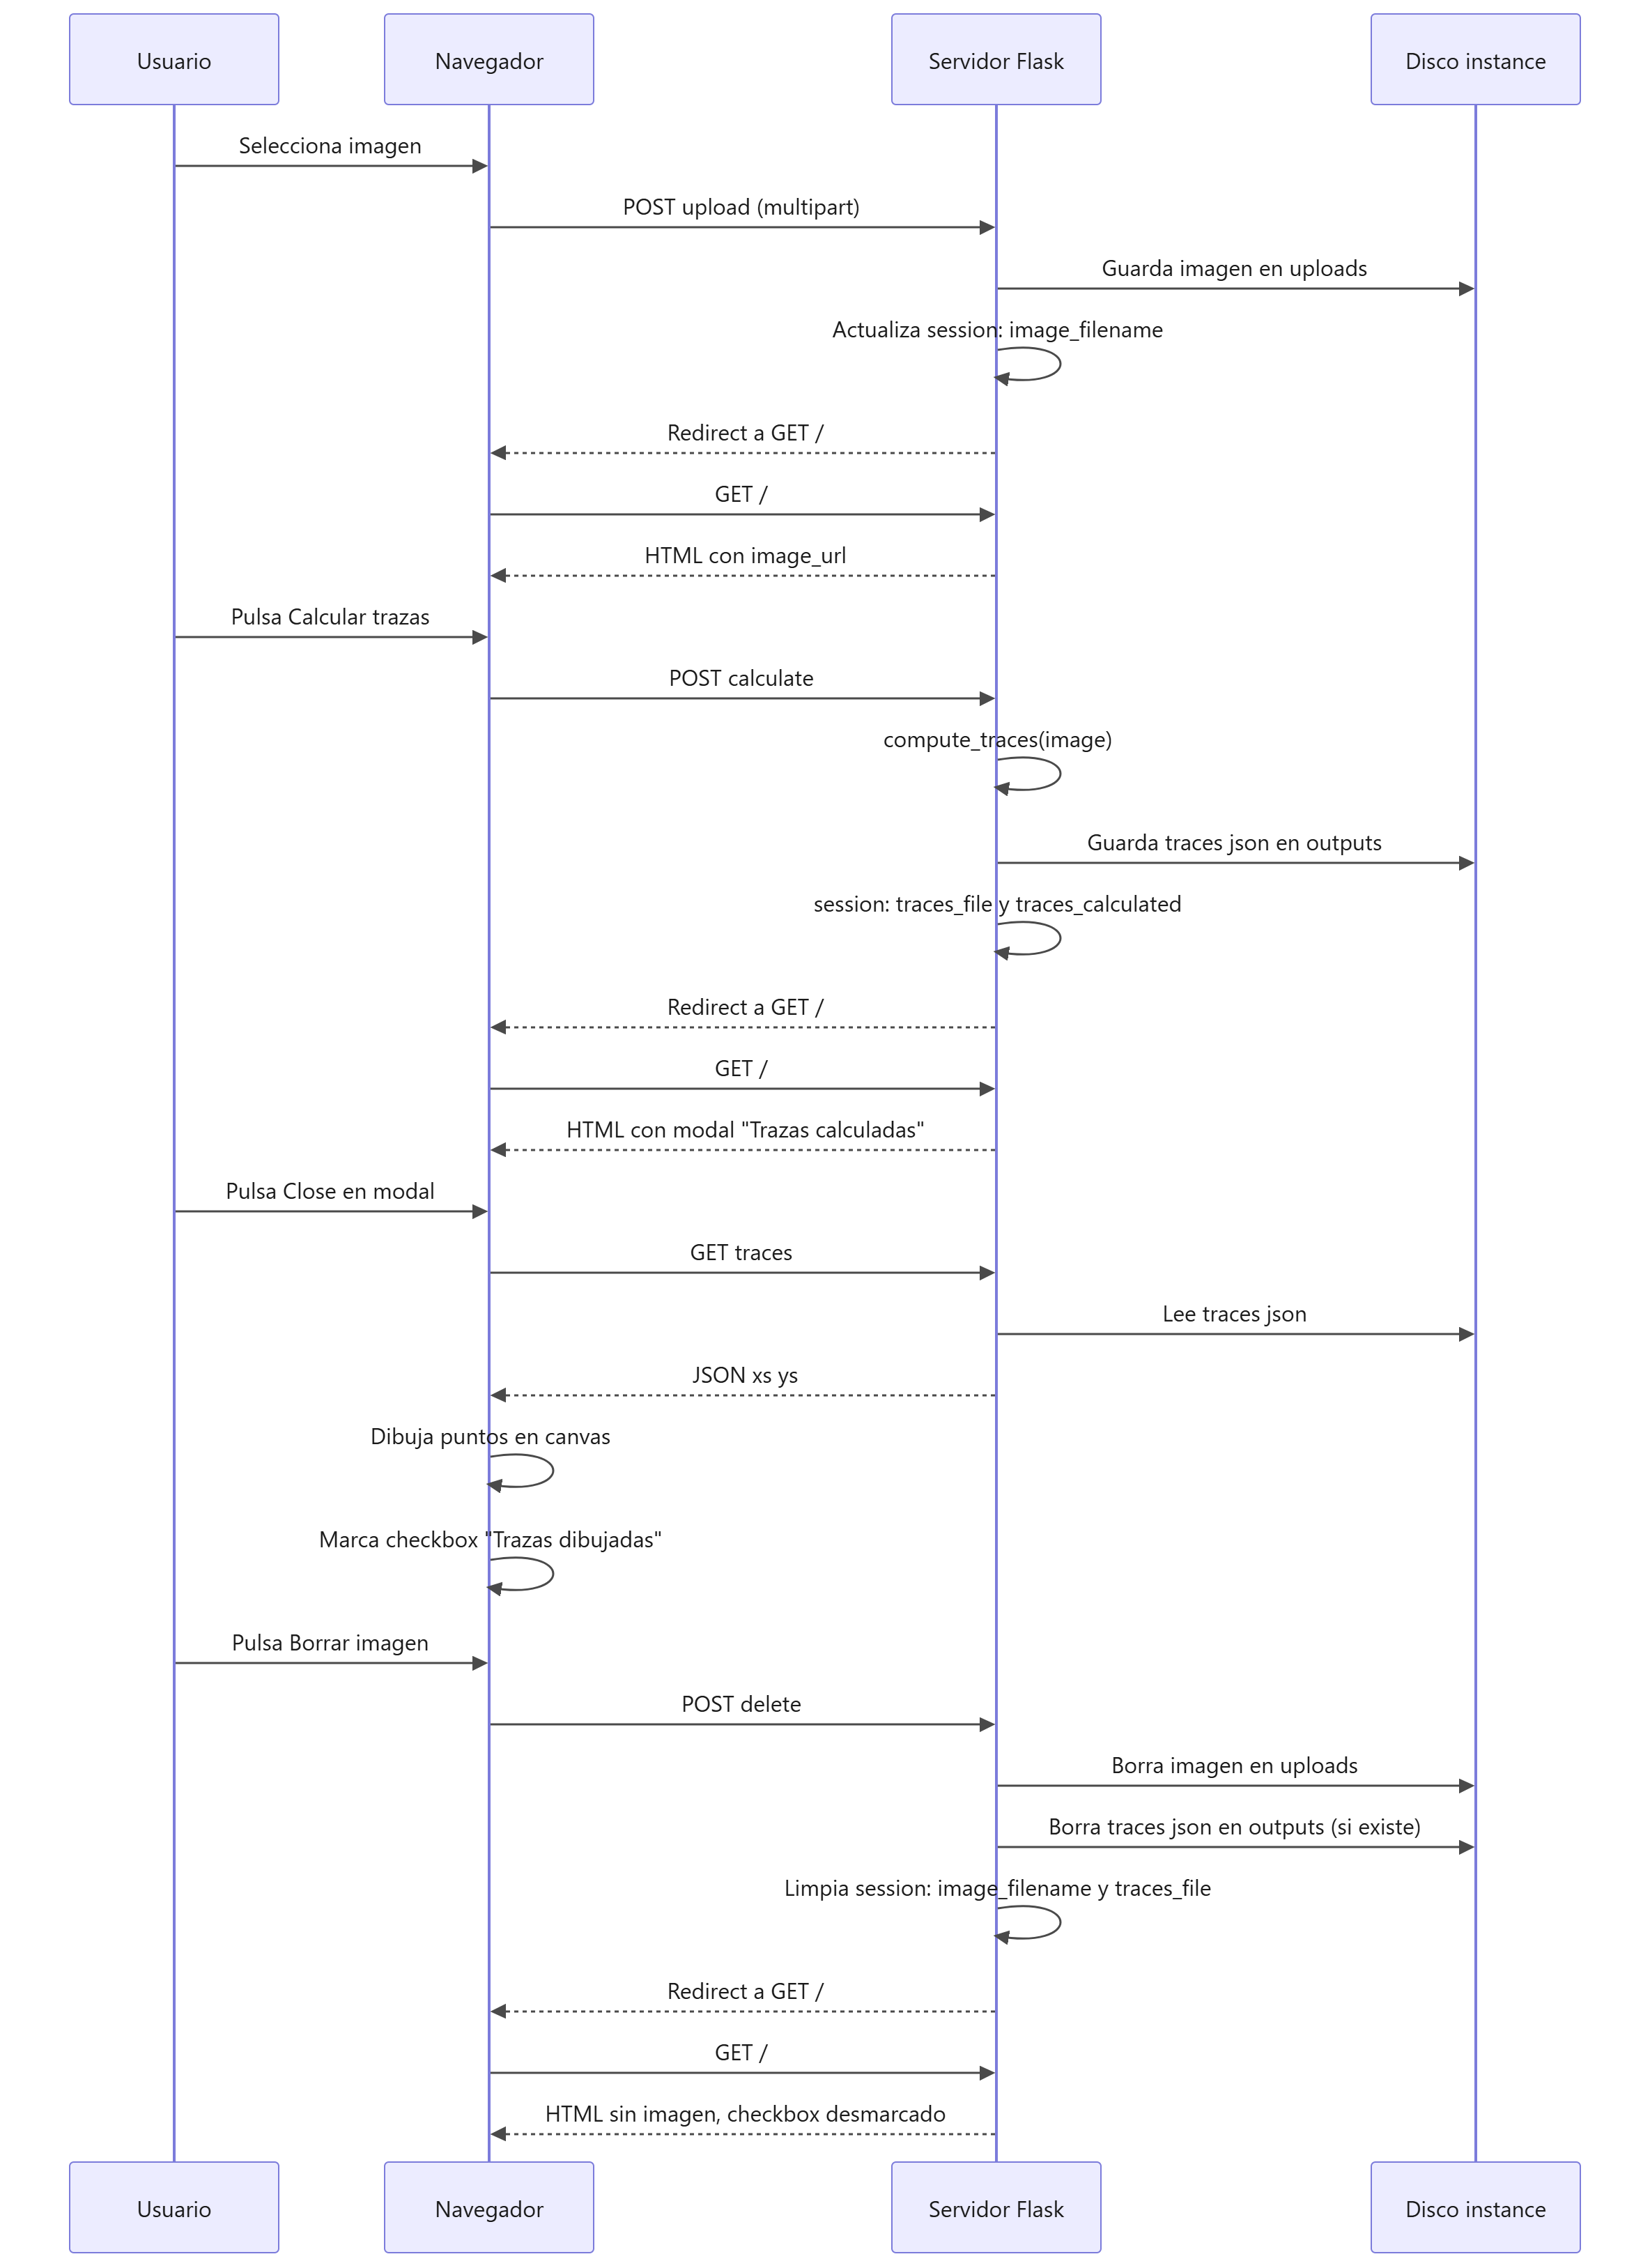
\includegraphics[width=0.7\linewidth]{img/diagrama_secuencia}
	\caption[Diagrama de Secuencia de la aplicación]{}
	\label{fig:diagramasecuencia}
\end{figure}

La Figura \ref{fig:diagramasecuencia} describe de forma cronológica el flujo de interacción entre el usuario, el navegador, el servidor Flask y el sistema de almacenamiento, permitiendo comprender el comportamiento dinámico de la aplicación.

El proceso se inicia cuando el usuario selecciona una imagen desde la interfaz. El navegador envía dicha imagen al servidor mediante una petición \textit{POST upload}, tras lo cual Flask la persiste en disco y actualiza el estado de la sesión. A continuación, el servidor responde con una redirección que provoca la recarga de la página principal, mostrando la imagen cargada.

Posteriormente, cuando el usuario solicita el cálculo de trazas, el servidor ejecuta la lógica correspondiente, genera los resultados en formato JSON y los almacena en el sistema de ficheros, actualizando de nuevo la sesión para reflejar el nuevo estado. La respuesta se materializa en una recarga de la interfaz que incluye un modal de confirmación.

Una vez cerrado el modal, el navegador solicita explícitamente los resultados mediante una petición \textit{GET traces}. El servidor lee el fichero JSON previamente generado y lo devuelve al cliente, donde el código JavaScript se encarga de dibujar las trazas sobre el \textit{canvas} y reflejar visualmente el estado de la aplicación.

Finalmente, si el usuario decide eliminar la imagen, se envía una petición \textit{POST delete}. El servidor elimina tanto la imagen como los resultados asociados, limpia la información de la sesión y devuelve la aplicación a su estado inicial mediante una nueva recarga de la página.


\section{Diseño procedimental}





